\documentclass[xcolor=x11names,compress]{beamer}

    %% General document %%%%%%%%%%%%%%%%%%%%%%%%%%%%%%%%%%
    \usepackage{graphicx}
    \graphicspath{{graphics/}}

    \usepackage{animate}
    \usepackage{tikz}
    \usetikzlibrary{calc, positioning, matrix, fit, backgrounds, chains}

    % \usepackage{pgfpages}
    % \usepackage[normalem]{ulem}
% magic to allow tikz nodes to use onslide
    \tikzset{onslide/.code args={<#1>#2}{%
    \only<#1>{\pgfkeysalso{#2}} % \pgfkeysalso doesn't change the path
    }}

    \usepackage{color,colortbl}
    \usepackage{framed}
    \usepackage{textcomp, setspace} %Needed for customization of ``listings''
    % package
    \usepackage[procnames]{listings} % to display code; don't forget [fragile]
    % option after \begin{frame}
    \input{inputs/rgb}
    \definecolor{shadecolor}{rgb}{1,.9,.3}
    
    \usepackage [autostyle]{csquotes}
    \MakeOuterQuote{"}
    
    \lstset{
        backgroundcolor=\color{shadecolor},
        tabsize=4,
        rulecolor=,
        language=python,
            basicstyle=\ttfamily\setstretch{1},
            upquote=true,
            aboveskip={1.5\baselineskip},
            columns=fixed,
            showstringspaces=false,
            extendedchars=true,
            breaklines=true,
            prebreak = \raisebox{0ex}[0ex][0ex]{\ensuremath{\hookleftarrow}},
            frame=single,
            showtabs=false,
            showspaces=false,
            showstringspaces=false,
            identifierstyle=\ttfamily,
            keywordstyle=\color[rgb]{0,0,1},
            commentstyle=\color[rgb]{0.133,0.545,0.133},
            stringstyle=\color[rgb]{0.627,0.126,0.941},
            numbers=left, 
            numberstyle=\tiny, 
            stepnumber=2, 
            numbersep=5pt
    }
    
    %%%%%%%%%%%%%%%%%%%%%%%%%%%%%%%%%%%%%%%%%%%%%%%%%%%%%%
    
    %% Beamer Layout %%%%%%%%%%%%%%%%%%%%%%%%%%%%%%%%%%
    \usetheme{Madrid}
    \usecolortheme{seahorse}
    \useoutertheme[subsection=false,shadow]{miniframes}
    \useinnertheme{default}
    % \usefonttheme{serif}
    \usepackage{palatino}
    
    \setbeamerfont{title like}{shape=\scshape}
    \setbeamerfont{frametitle}{shape=\scshape, series = \bfseries}
    \setbeamertemplate{frametitle}[default][center]
    \setbeamertemplate{headline}{} %suppress headline (navigation pane)
    
    \setbeamertemplate{footline}
    {
      \leavevmode%
      \hbox{
      \begin{beamercolorbox}[wd=.1\paperwidth,ht=2.2ex,dp=1ex,center]{author in head/foot}
        \usebeamerfont{author in head/foot}\insertshortauthor
      \end{beamercolorbox}
      \begin{beamercolorbox}[wd=.8\paperwidth,ht=2.2ex,dp=1ex,center]{title in head/foot}%
        \usebeamerfont{title in head/foot}\insertshorttitle\hspace*{3em}
      \end{beamercolorbox}}
      \begin{beamercolorbox}[wd=.05\paperwidth,ht=2.2ex,dp=1ex,center]{}
         \insertframenumber{} / \inserttotalframenumber\hspace*{-3ex}
      \end{beamercolorbox}
    }
    
    
    \renewcommand{\(}{\begin{columns}}
    \renewcommand{\)}{\end{columns}}
    \newcommand{\<}[1]{\begin{column}{#1}}
    \renewcommand{\>}{\end{column}}
    
    \def\signed #1{{\leavevmode\unskip\nobreak\hfil\penalty50\hskip2em
      \hbox{}\nobreak\hfil(#1)%
      \parfillskip=0pt \finalhyphendemerits=0 \endgraf}}
    
    \newsavebox\mybox
    \newenvironment{aquote}[1]
      {\savebox\mybox{#1}\begin{quote}}
      {\signed{\usebox\mybox}\end{quote}}
    %%%%%%%%%%%%%%%%%%%%%%%%%%%%%%%%%%%%%%%%%%%%%%%%%%%%
    \title{Linear models}
\author[Samraat]{Samraat Pawar}
\institute{{\it Department of Life Sciences (Silwood Park)}\\
  \vspace{12pt}
  \centering
  
\includegraphics[height = .3in]{graphics/Imperial_Color1.pdf}
}
\date{}


%%%%%%%%%%%%%%%%%%%%%%%%%%%%%%%%%%%%%%%%%%%%%%%%%%%%
%%%%%%%%%%%%%%%%%%%%%%%%%%%%%%%%%%%%%%%%%%%%%%%%%%%%
\begin{document}

%%%%%%%%%%%%%%%%%%%%%%%%%%%%%%%%%%%%%%%%%%%%%%%%%%%%%%%%%%%%%%%%%%%%%
\begin{frame}

\titlepage
    
\end{frame}

%%%%%%%%%%%%%%%%%%%%%%%%%%%%%%%%%%%%%%%%%%%%%%%%%%%%%%%%%%%%%%%%%%%%%
\begin{frame}{Lecture Outline}

Topics:
\begin{itemize}
    \item What is a linear model?
    \begin{itemize}
        \item Regression
        \item ANOVA
        \item Multiple explanatory variables (ANCOVA)
    \end{itemize} 
    \item Fitting linear models to your data  
    \item Is the fitted linear model appropriate for the data?
    \item How well does a fitted linear model explain the data?
    \end{itemize}
  
    \pause
    \vspace{12pt}
    Concepts:
   \begin{itemize}
    \item Types of variable: continuous versus categorical 
    \item Terms and coefficients of a model
    \item Model fitting and model residuals
    \item Significance testing and p-values
   \end{itemize}
  
  \end{frame}
  
  %%%%%%%%%%%%%%%%%%%%%%%%%%%%%%%%%%%%%%%%%%%%%%%%%%%%%%%%%%%%%%%%%%%%%
  \section{What is a linear model?}
  
  %%%%%%%%%%%%%%%%%%%%%%%%%%%%%%%%%%%%%%%%%%%%%%%%%%%%%%%%%%%%%%%%%%%%%
  \begin{frame}{What predicts the weights ($w$) of lecturers?}
  
  Use {\it intuition} and {\it prior knowledge} to identify the {\it variables} to collect...
  \begin{itemize}[<+->]
  
      \item Height ($h$) in metres
      \item Exercise per week ($e$) in hours
      \item Gender ($g$)
      \item Distance from home to nearest Greggs bakery ($d$) in metres
      \item Ownership of a games console ($c$)
  
  \pause
  \end{itemize}
  \vspace{12pt}
  \ldots and build a mathematical model:\\
  \vspace{6pt}
  Lecturer weight ($w$) = {\it Combination} of {\it Independent Variables} (that determine $w$)
  \pause
  $$w = \beta_1 + \beta_2 h + \beta_3 e + \beta_4 g_m  + \beta_5 d + \beta_6 c_s + \beta_7 c_a + \varepsilon$$
  
\end{frame}

%%%%%%%%%%%%%%%%%%%%%%%%%%%%%%%%%%%%%%%%%%%%%%%%%%%%%%%%%%%%%%%%%%%%
\begin{frame}{The linear model}

    A combination of four components:

    \begin{center}
    
    %% Fix the equation in place on the slide 
    %% - avoid absolute tikz positions because the overlay makes it hard to 
    %%   get the rest of the slide aligning correctly.
    %% - using a bounding box forces the underlying text down to the same level
    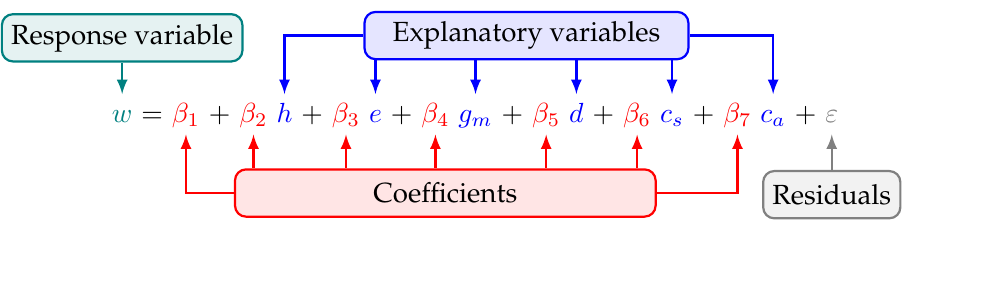
\begin{tikzpicture} 
    
    \useasboundingbox (0 mm, 0mm) rectangle (118 mm, 30mm); % width of slide less margins - fixed (128 - 2 x 5)
    
    % style fix minimum height on nodes to align labels above components, 
    % a chain to align the equation along and some colour styles for overlays
    \begin{scope}[every node/.style={text height=3mm,  text depth=1mm, on chain, inner sep=0.5mm},
                  gr/.style={teal}, 
                  rd/.style={red}, 
                  bl/.style={blue}, 
                  gy/.style={gray},
                  start chain, node distance=0mm]
    
    \node [gr] (w) at (12mm, 19mm) {$w$}; % fixed position within bbox
    \node      (eq) {$=$};
    \node [rd] (b1) {$\beta_1$};
    \node      (p)  {$+$};
    \node [rd] (b2) {$\beta_2$};
    \node [bl] (h)  {$h$};
    \node      (p)  {$+$};
    \node [rd] (b3) {$\beta_3$};
    \node [bl] (e)  {$e$};
    \node      (p)  {$+$};
    \node [rd] (b4) {$\beta_4$};
    \node [bl] (g)  {$g_m$};
    \node      (p)  {$+$};
    \node [rd] (b5) {$\beta_5$};
    \node [bl] (d)  {$d$};
    \node      (p)  {$+$};
    \node [rd] (b6) {$\beta_6$};
    \node [bl] (cS)  {$c_s$};
    \node      (p)  {$+$};
    \node [rd] (b7) {$\beta_7$};
    \node [bl] (cA)  {$c_a$};
    \node      (p)  {$+$};
    \node [gy] (eps)  {$\varepsilon$};
    
    
    \end{scope}
    
    \begin{scope}[every node/.style={rounded corners, draw, minimum height=6mm},
                  every path/.style={latex-, draw=red, thick}]
                  
        \node (exp)  [inner sep=0pt, yshift=1cm, fit={(e) (cS)}, label=center:Explanatory variables, fill=blue!10, draw=blue] {};	
        \node (coef) [inner sep=0pt, yshift=-1cm, fit={(b2) (b6)}, label=center:Coefficients, fill=red!10, draw=red] {};	
        \node (resp)  [above = 4mm of w, fill=teal!10, draw=teal] {Response variable};
        \node (resid)  [below = 4.5mm of eps, fill=gray!10, draw=gray] {Residuals};
    
        \foreach \i in {e, d, g, cS}  \draw [blue] (\i.north) -- (\i.north |- exp.south);
        \draw [blue] (cA.north) |- (exp.east);
        \draw [blue] (h.north) |- (exp.west);	
        \foreach \i in {b2, b3, b4, b5, b6}  \draw [red] (\i.south) -- (\i.south |- coef.north);
        \draw [red] (b7.south) |- (coef.east);
        \draw [red] (b1.south) |- (coef.west);
        \draw [teal] (w.north) --  (resp.south);
        \draw [gray] (eps.south) -- (resid.north);
    
        
    \end{scope}
    
    \end{tikzpicture}
    
    
    \begin{itemize}
    \item A \textcolor{teal}{response variable} ($w$)
    \item A set of \textcolor{blue}{explanatory variables} ($h,e,g,d,c$)
    \item A set of \textcolor{red}{coefficients} ($\beta_1$ -- $\beta_7$)
    \item A set of \textcolor{gray}{residuals} ($\varepsilon$)
    \end{itemize}
    
    \end{center}
    \end{frame}

%%%%%%%%%%%%%%%%%%%%%%%%%%%%%%%%%%%%%%%%%%%%%%%%%%%%%%%%%%%%%%%%%%%%%
\begin{frame}[t]{The Variables}
    
    \begin{center}
    \begin{tikzpicture} 
    
    \useasboundingbox (0 mm, 0mm) rectangle (118 mm, 30mm); % width of slide less margins - fixed (128 - 2 x 5)
    
    % style fix minimum height on nodes to align labels above components, 
    % a chain to align the equation along and some colour styles for overlays
    \begin{scope}[every node/.style={text height=3mm,  text depth=1mm, on chain, inner sep=0.5mm},
                  gr/.style={teal}, 
                  rd/.style={red}, 
                  bl/.style={blue}, 
                  gy/.style={gray},
                  start chain, node distance=0mm]
    
    \node [bl] (w) at (12mm, 19mm) {$w$}; % fixed position within bbox
    \node      (eq) {$=$};
    \node [gy] (b1) {$\beta_1$};
    \node      (p)  {$+$};
    \node [gy] (b2) {$\beta_2$};
    \node [bl] (h)  {$h$};
    \node      (p)  {$+$};
    \node [gy] (b3) {$\beta_3$};
    \node [bl] (e)  {$e$};
    \node      (p)  {$+$};
    \node [gy] (b4) {$\beta_4$};
    \node [rd] (g)  {$g_m$};
    \node      (p)  {$+$};
    \node [gy] (b5) {$\beta_5$};
    \node [bl] (d)  {$d$};
    \node      (p)  {$+$};
    \node [gy] (b6) {$\beta_6$};
    \node [rd] (cS)  {$c_s$};
    \node      (p)  {$+$};
    \node [gy] (b7) {$\beta_7$};
    \node [rd] (cA)  {$c_a$};
    \node [gy] (p)  {$+$};
    \node [gy] (eps)  {$\varepsilon$};
    
    
    \end{scope}
    
    \begin{scope}[every node/.style={rounded corners, draw, minimum height=6mm},
                  every path/.style={latex-, draw=red, thick}]
                  
        \node (cont)  [inner sep=0pt, yshift=1cm, fit={(w) (d)}, label=center:Continuous variables, fill=blue!10, draw=blue] {};	
        \node (cat) [inner sep=0pt, yshift=-1cm, fit={(g) (cA)}, label=center:Categorical variables, fill=red!10, draw=red] {};	
    
        \foreach \i in {w, h, e, d}  \draw [blue] (\i.north) -- (\i.north |- exp.south);   
        \foreach \i in {g, cA, cS}  \draw [red] (\i.south) -- (\i.south |- coef.north);   
        
    \end{scope}
    
    \end{tikzpicture}
    
    \begin{itemize}[<+->]\itemsep6pt
    \item The response variable is always \textcolor{blue}{continuous}.
    \item The explanatory variables can be a mix of:
    \begin{itemize}
    \item \textcolor{blue}{Continuous} variables: height, exercise and distance.
    \item \textcolor{red}{Categorical} variables: gender and console ownership.
    \end{itemize}
    \item \textcolor{red}{Categorical} variables or {\it factors} have a number of {\it levels}:
    
    \begin{itemize}
      \item Gender has two levels (Male / Female)
        \item Console has three levels (None / Sofa-based / Active)
    \end{itemize}
  
    \end{itemize}
 \end{center}
\end{frame}

%%%%%%%%%%%%%%%%%%%%%%%%%%%%%%%%%%%%%%%%%%%%%%%%%%%%%%%%%%%%%%%%%%%%%
\begin{frame}{The Terms and Coefficients}
    
    \begin{center}
    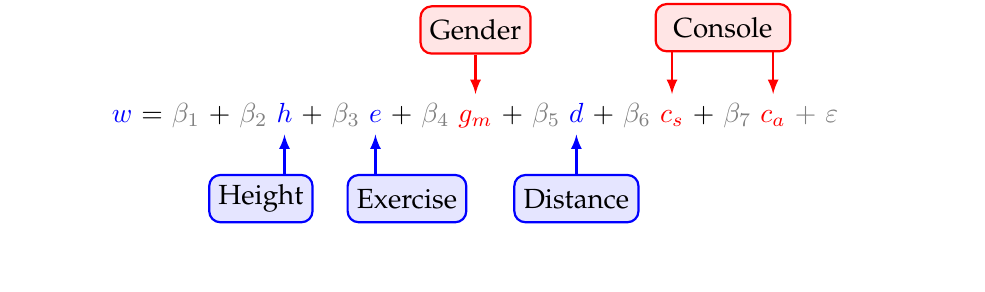
\begin{tikzpicture} 
    
    \useasboundingbox (0 mm, 0mm) rectangle (118 mm, 30mm); % width of slide less margins - fixed (128 - 2 x 5)
    
    % style fix minimum height on nodes to align labels above components, 
    % a chain to align the equation along and some colour styles for overlays
    \begin{scope}[every node/.style={text height=3mm,  text depth=1mm, on chain, inner sep=0.5mm},
                  gr/.style={teal}, 
                  rd/.style={red}, 
                  bl/.style={blue}, 
                  gy/.style={gray},
                  start chain, node distance=0mm]
    
    \node [bl] (w) at (12mm, 19mm) {$w$}; % fixed position within bbox
    \node      (eq) {$=$};
    \node [gy] (b1) {$\beta_1$};
    \node      (p)  {$+$};
    \node [gy] (b2) {$\beta_2$};
    \node [bl] (h)  {$h$};
    \node      (p)  {$+$};
    \node [gy] (b3) {$\beta_3$};
    \node [bl] (e)  {$e$};
    \node      (p)  {$+$};
    \node [gy] (b4) {$\beta_4$};
    \node [rd] (g)  {$g_m$};
    \node      (p)  {$+$};
    \node [gy] (b5) {$\beta_5$};
    \node [bl] (d)  {$d$};
    \node      (p)  {$+$};
    \node [gy] (b6) {$\beta_6$};
    \node [rd] (cS)  {$c_s$};
    \node      (p)  {$+$};
    \node [gy] (b7) {$\beta_7$};
    \node [rd] (cA)  {$c_a$};
    \node [gy] (p)  {$+$};
    \node [gy] (eps)  {$\varepsilon$};
    
    
    \end{scope}
    
    \begin{scope}[every node/.style={rounded corners, draw, minimum height=6mm},
                  every path/.style={latex-, draw=red, thick}]
                  
        \node (height)    [below=0.5cm of h, fill=blue!10, draw=blue, xshift=-3mm] {Height};
        \draw [blue] (h.south) -- (h.south |- height.north);
    
        \node (exercise)  [below=0.5cm of e, fill=blue!10, draw=blue, xshift=4mm] {Exercise};
        \draw [blue] (e.south) -- (e.south |- exercise.north);
    
        \node (distance)  [below=0.5cm of d, fill=blue!10, draw=blue] {Distance};
        \draw [blue] (d.south) -- (d.south |- distance.north);
    
        \node (gender)  [above=0.5cm of g, fill=red!10, draw=red] {Gender};
        \draw [red] (g.north) -- (g.north |- gender.south);
    
        \node (console) [inner sep=0pt, yshift=1.1cm, fit={(cA) (cS)}, label=center:Console, fill=red!10, draw=red] {};	
        \foreach \i in {cA, cS}  \draw [red] (\i.north) -- (\i.north |- console.south);   
        
    \end{scope}
    
    \end{tikzpicture}
    
    
    \begin{itemize}[<+->]\itemsep6pt
    \item Each explanatory variable is a {\it term} in the model
    \item Each term has at least one coefficient
    \item \textcolor{blue}{Continuous} terms always have one coefficient
    \item Categorical \textcolor{red}{Factors} have $N - 1$ coefficients, where $N$ is the number of levels ({\it where are the missing coefficients??})
    
    \end{itemize}
    \end{center}
\end{frame}

%%%%%%%%%%%%%%%%%%%%%%%%%%%%%%%%%%%%%%%%%%%%%%%%%%%%%%%%%%%%%%%%%%%%%
\begin{frame}{Wait! Why $N-1$ Coefficients? What is $\beta_1$?}
    
    \begin{center}
    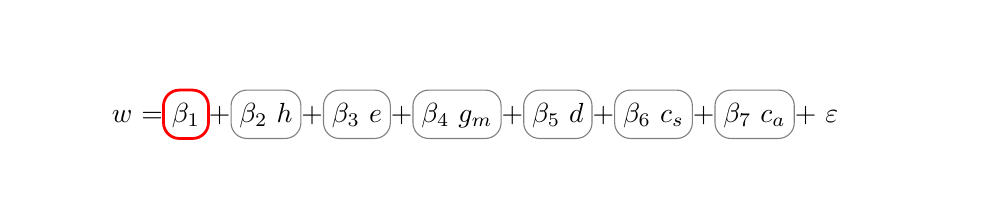
\begin{tikzpicture}[every node/.style={text height=3mm,  text depth=1mm, on chain, inner sep=0.5mm},
                  gr/.style={teal}, 
                  rd/.style={red}, 
                  bl/.style={blue}, 
                  gy/.style={gray},
                  pr/.style={draw, rounded corners=2mm, gray},
                  start chain, node distance=0mm]
    
    \useasboundingbox (0 mm, 0mm) rectangle (118 mm, 21mm); % width of slide less margins - fixed (128 - 2 x 5)
    
    \node  (w) at (12mm, 10mm) {$w$}; % fixed position within bbox
    \node  (eq) {$=$};
    \node  (b1) {$\beta_1$};
    \node  (p)  {$+$};
    \node  (b2) {$\beta_2$};
    \node  (h)  {$h$};
    \node  (p)  {$+$};
    \node  (b3) {$\beta_3$};
    \node  (e)  {$e$};
    \node  (p)  {$+$};
    \node  (b4) {$\beta_4$};
    \node  (g)  {$g_m$};
    \node  (p)  {$+$};
    \node  (b5) {$\beta_5$};
    \node  (d)  {$d$};
    \node  (p)  {$+$};
    \node  (b6) {$\beta_6$};
    \node  (cS)  {$c_s$};
    \node  (p)  {$+$};
    \node  (b7) {$\beta_7$};
    \node  (cA)  {$c_a$};
    \node  (p)  {$+$};
    \node  (eps)  {$\varepsilon$};
    
    \node [pr, red, fit= (b1), line width=1pt] {};
    \node [pr, fit= (b2) (h)] {};
    \node [pr, fit= (b3) (e)] {};
    \node [pr, fit= (b4) (g)] {};
    \node [pr, fit= (b5) (d)] {};
    \node [pr, fit= (b6) (cS)] {};
    \node [pr, fit= (b7) (cA)] {};
    
    \end{tikzpicture}
    %
    
    \begin{itemize}[<+->]\itemsep6pt
    \item Two ways of thinking about $\beta_1$:
    \begin{itemize}
    \item Continuous variables: the $y$ {\it intercept}
    \item Factors: the baseline or {\it reference} value
    \end{itemize}
    \item This baseline is the value for the {\it first levels} of each factor
    \item All response values start at this baseline
    \item All the other coefficients measure {\it differences} from $\beta_1$:
    \begin{itemize}
    \item along a continuous slope
    \item as an offset to a different level
    \end{itemize}
    \end{itemize}
    
    \end{center}
    
    \end{frame}
 
 %%%%%%%%%%%%%%%%%%%%%%%%%%%%%%%%%%%%%%%%%%%%%%%%%%%%%%%%%%%%%%%%%%%%%

\begin{frame}{So, to put it simply,}

Linear models are just a sum of {\it terms} that are {\it linear} in the {\it coefficients}:
\vspace{-20pt}
\begin{center}
    \begin{tikzpicture}[every node/.style={text height=3mm,  text depth=1mm, on chain, inner sep=0.5mm},
                cross/.style={path picture={
                    \draw[red, ultra thick] (path picture bounding box.center) +(0, 1.4mm) -- +(0, -1.4mm) (path picture bounding box.center) +(1.4mm, 0mm) -- +(-1.4mm,0) ;}},
                gr/.style={teal}, 
                rd/.style={cross, red}, 
                bl/.style={blue}, 
                gy/.style={gray},
                pr/.style={draw, rounded corners=2mm, gray},
                start chain, node distance=0mm]

    \useasboundingbox (0 mm, 0mm) rectangle (118 mm, 21mm); % width of slide less margins - fixed (128 - 2 x 5)

    \node      (w) at (12mm, 10mm) {$w$}; % fixed position within bbox
    \node      (eq) {$=$};
    \node      (b1) {$\beta_1$};
    \node [rd] (p)  {$+$};
    \node      (b2) {$\beta_2$};
    \node      (h)  {$h$};
    \node [rd] (p)  {$+$};
    \node      (b3) {$\beta_3$};
    \node      (e)  {$e$};
    \node [rd] (p)  {$+$};
    \node      (b4) {$\beta_4$};
    \node      (g)  {$g_m$};
    \node [rd] (p)  {$+$};
    \node      (b5) {$\beta_5$};
    \node      (d)  {$d$};
    \node [rd] (p)  {$+$};
    \node      (b6) {$\beta_6$};
    \node      (cS)  {$c_s$};
    \node [rd] (p)  {$+$};
    \node      (b7) {$\beta_7$};
    \node      (cA)  {$c_a$};
    \node [rd] (p)  {$+$};
    \node      (eps)  {$\varepsilon$};

    \end{tikzpicture}
    
\end{center}
\vspace{-20pt}

\pause 
What our example linear model means (literally):
\begin{itemize}[<+->]\itemsep6pt
\item The coefficient $\beta_1$ is the baseline value of {\it weight} for {\it women} with {\it no games console}
\item The model tells us how much (determined by the other coefficients) to add to this baseline weight \ldots
    \begin{itemize}
        \item  for a height of 1.82 metres?
        \item  for doing 150 minutes of exercise a week?
        \item  for being male?
        \item  for living 2416 metres from a Greggs?
        \item  for owning an Xbox?
    \end{itemize}
\end{itemize}
    
\end{frame}

%%%%%%%%%%%%%%%%%%%%%%%%%%%%%%%%%%%%%%%%%%%%%%%%%%%%%%%%%%%%%

\begin{frame}{Examples of Linear Models}

    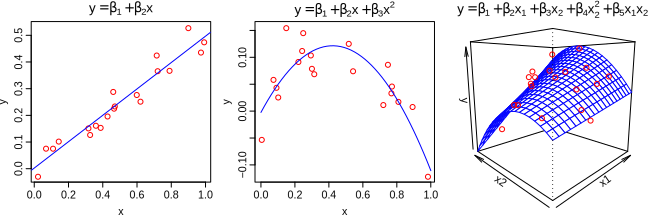
\includegraphics[width=\textwidth]{Linear.pdf}
    
    \begin{itemize}\itemsep10pt
    \item These are {\it all} linear models (fitted to data)
    \item Each model a {\it sum} of {\it terms} that are {\it linear in coefficients}
    \item {\it Linear models can include curved relationships (e.g. polynomials) --- this is a common point of confusion!}
    \end{itemize}
    
    \end{frame}
    
%%%%%%%%%%%%%%%%%%%%%%%%%%%%%%%%%%%%%%%%%%%%%%%%%%%%%%%%%%%%%%%%%%%%%

\begin{frame}{Linear model with one continuous variable}

    \begin{columns}[T]
    
        \column{0.5\textwidth}
            \includegraphics[width=\textwidth]{Origin.pdf}
            
        \column{0.5\textwidth}
            \begin{align*}
              y  &=  \beta_1 x \\
              \\
              4  &=  4 \times 1 \\
              8  &=  4 \times 2 \\
              12 &=  4 \times 3 \\
              16 &=  4 \times 4   
            \end{align*}
            \[\beta_1 =4\]
    \end{columns}

\pause

\begin{center}
    {\bf Regression} with {\it known baseline value (intercept) }
\end{center}

\end{frame}

    %%%%%%%%%%%%%%%%%%%%%%%%%%%%%%%%%%%%%%%%%%%%%%%%%%%%%%%%%%%%%%%%%%%%%
    \begin{frame}{Linear model with one continuous variable}
    
    \begin{columns}[T]
    
        \column{0.5\textwidth}
            \includegraphics[width=\textwidth]{Intercept.pdf}
            
        \column{0.5\textwidth}
            \begin{align*}
              y  &= \beta_1 + \beta_2 x \\
              \\
              9  &= 5 + 4 \times 1 \\
              13 &= 5 + 4 \times 2 \\
              17 &= 5 + 4 \times 3 \\
              21 &= 5 + 4 \times 4   
            \end{align*}
            \[\beta_1 = 5; \beta_2=4\]
    \end{columns}
\pause
    \begin{center}
        {\bf Regression} with {\it unknown baseline value (intercept) }
    \end{center}
    
\end{frame}

%%%%%%%%%%%%%%%%%%%%%%%%%%%%%%%%%%%%%%%%%%%%%%%%%%%%%%%%%%%%%%%%%%%%%
\begin{frame}{Linear model with one factor (categorical variable)}

    \begin{columns}[T]
    
        \column{0.5\textwidth}
            \includegraphics[width=\textwidth]{Factor.pdf}
            
        \column{0.5\textwidth}
            \begin{align*}
              y  &= \beta_1 + \beta_2 g_m  \\
              \\
              2  &= 2 + 3 \times 0 \\
              2  &= 2 + 3 \times 0 \\
              2  &= 2 + 3 \times 0 \\
              5  &= 2 + 3 \times 1 \\  
              5  &= 2 + 3 \times 1 \\
              5  &= 2 + 3 \times 1
            \end{align*}
            \[\beta_1 = 2; \beta_2=3\]
    \end{columns}
    \pause
    \begin{center}
        {\it Analysis of Variance} ({\bf ANOVA})
    \end{center}

\end{frame}
    
%%%%%%%%%%%%%%%%%%%%%%%%%%%%%%%%%%%%%%%%%%%%%%%%%%%%%%%%%%%%%%%%%%%%%
\begin{frame}{Linear model with one continuous variable and one factor}

    \begin{columns}[T]
    
        \column{0.5\textwidth}
            \includegraphics[width=\textwidth]{TwoVars.pdf}
            
        \column{0.5\textwidth}
            \begin{align*}
              y  &= \beta_1  + \beta_2 x + \beta_3 g_m\\
              \\
              3   &= 1 + 2 \times 1 + 3 \times 0\\
              5   &= 1 + 2 \times 2 + 3 \times 0\\
              7   &= 1 + 2 \times 3 + 3 \times 0\\
              6   &= 1 + 2 \times 1 + 3 \times 1\\  
              8   &= 1 + 2 \times 2 + 3 \times 1\\
              10  &= 1 + 2 \times 3 + 3 \times 1
            \end{align*}
            \[\beta_1 = 1; \beta_2=2; \beta_3=3\]
    \end{columns}
    \pause
    \begin{center}
        {\it Multiple Expanatory variables, Analysis of Covariance} ({\bf ANCOVA})
    \end{center}
\end{frame}
   
%%%%%%%%%%%%%%%%%%%%%%%%%%%%%%%%%%%%%%%%%%%%%%%%%%%%%%%%%%%%%%%%%%%%%
\begin{frame}{Closer look at the ANCOVA example}

    \begin{columns}[T]
    
        \column{0.5\textwidth}
            \includegraphics[width=\textwidth]{TwoVarsHighlight.pdf}
            
            \column{0.5\textwidth}
                \begin{align*}
                  y  &= \beta_1  + \beta_2 x + \beta_3 g_m\\
                  \\
                  3   & = 1 + 2 \times 1 + 3 \times 0\\
                  5   & = 1 + 2 \times 2 + 3 \times 0\\
                  7   & = 1 + 2 \times 3 + 3 \times 0\\
                  6   & = 1 + 2 \times 1 + 3 \times 1\\  
                  {\color{red}8} & {\color{red}\;= 1 + 2 \times 2 + 3 \times 1}\\ % loses a space for some reason
                  10  & = 1 + 2 \times 3 + 3 \times 1
                \end{align*}
                \[\beta_1 = 1; \beta_2=2; \beta_3=3\]
    \end{columns}
    \end{frame}
    
%%%%%%%%%%%%%%%%%%%%%%%%%%%%%%%%%%%%%%%%%%%%%%%%%%%%%%%%%%%%%%%%%%%%%
\section{Fitting a LM}

%%%%%%%%%%%%%%%%%%%%%%%%%%%%%%%%%%%%%%%%%%%%%%%%%%%%%%%%%%%%%%%%%%%%%

\begin{frame}{``Fitting'' a linear model to data}

% Residuals; variation is everywhere!
% \pause

 \begin{center}
            \includegraphics[width=0.5\textwidth]{CarnivoreBMRplot.pdf}\\
            \vspace{-6pt}
            {\tiny Rizzuto et al. 2017, Nat Ecol Evol}
\end{center}		
\begin{itemize}\itemsep6pt
    \item Data always shows variation from a perfect model (deviations)
    \begin{itemize}[<+->]
    \item Missing variables (age, lab vs. field biology, time of day) 
    \item Measurement error 
    \item Stochastic variation
    \end{itemize}
    \end{itemize}

\end{frame}
    
    
%%%%%%%%%%%%%%%%%%%%%%%%%%%%%%%%%%%%%%%%%%%%%%%%%%%%%%%%%%%%%%%%%%%%%
\begin{frame}{Fitting a Linear Model to Data}

    \begin{columns}[T]
    
        \column{0.5\textwidth}
            \includegraphics[width=\textwidth]{Error.pdf}
            
        \column{0.5\textwidth}
            
        \begin{center}
            {\it What line best passes through (describes) these data?}
           \end{center}
           \pause
           \begin{align*}
              y  &= \beta_1 + \beta_2 x \\
            \end{align*}
            \pause
            \vspace{-40pt}
            \begin{align*}
               9.50  &= \;?\; + \;?\; \times 1 \\
              11.00 &= \;?\; + \;?\; \times 2 \\
              19.58 &= \;?\; + \;?\; \times 3 \\
              20.00 &= \;?\; + \;?\; \times 4   
            \end{align*}
             
    \end{columns}
    \end{frame}
    
%%%%%%%%%%%%%%%%%%%%%%%%%%%%%%%%%%%%%%%%%%%%%%%%%%%%%%%%%%%%%%%%%%%%%

\begin{frame}{Fitting a Linear Model to Data: Guess}
    \begin{columns}[T]
   
       \column{0.5\textwidth}
           \includegraphics[width=\textwidth]{TooFlat.pdf}
           
       \column{0.5\textwidth}
           \begin{align*}
             y  &= \beta_1 + \beta_2 x  + {\color{red} \varepsilon }\\
             \\
             9.50  &= 12.52 + 1 \times 1 - {\color{red} 4.02}\\
             11.00 &= 12.52 + 1 \times 2 - {\color{red} 3.52}\\
             19.58 &= 12.52 + 1 \times 3 + {\color{red} 4.06}\\
             20.00 &= 12.52 + 1 \times 4 + {\color{red} 3.48} 
           \end{align*}
           \[\beta_1 = 12.52; \beta_2=1\]
   
   \end{columns}
   \end{frame}

%%%%%%%%%%%%%%%%%%%%%%%%%%%%%%%%%%%%%%%%%%%%%%%%%%%%%%%%%%%%%%%%%%%%%

\begin{frame}{Fitting a Linear Model to Data: Guess again!}
    \begin{columns}[T]

	\column{0.5\textwidth}
		\includegraphics[width=\textwidth]{TooSteep.pdf}
		
	\column{0.5\textwidth}
		\begin{align*}
		  y  &= \beta_1 + \beta_2 x + {\color{red} \varepsilon }\\
		  \\
		  9.50  &= -2.48 + 7 \times 1 + {\color{red} 4.98}\\
		  11.00 &= -2.48 + 7 \times 2 - {\color{red} 0.52}\\
		  19.58 &= -2.48 + 7 \times 3 + {\color{red} 1.06}\\
		  20.00 &= -2.48 + 7 \times 4 - {\color{red} 5.52} 
		\end{align*}
		\[\beta_1 = -2.48; \beta_2=7\]

\end{columns}		
\pause
\begin{center}
    {\it There must be a better way to do this!}
\end{center}

\end{frame}

%%%%%%%%%%%%%%%%%%%%%%%%%%%%%%%%%%%%%%%%%%%%%%%%%%%%%%%%%%%%%%%%%%%%%
\begin{frame}{Fitting a Linear Model: Least squares solution}

Minimize the {\it sum} of the {\it squared} {\it residuals:}

% %% animate directly from a multipage pdf - this is rather sweet!
% %% this is also over-engineered using timeline to only embed the axes once!
\begin{columns}[T]
\column{\textwidth}
\animategraphics[width=\textwidth, controls, %autoplay, %palindrome, 
                %  timeline=Varying_timeline.txt,
                 buttonsize=1em]{12}{Varying}{}{}

\end{columns}
\end{frame}

%%%%%%%%%%%%%%%%%%%%%%%%%%%%%%%%%%%%%%%%%%%%%%%%%%%%%%%%%%%%%
\begin{frame}{The (Ordinary) Least Squares fitting solution}

\begin{columns}[T]

	\column{0.5\textwidth}
		\includegraphics[width=\textwidth]{JustRight.pdf}
		
	\column{0.5\textwidth}
		\begin{align*}
		  y  &= \beta_1 + \beta_2 x  + {\color{red} \varepsilon }\\
		  \\
		  9.50  &= 5 + 4 \times 1 + {\color{red} 0.50}\\
		  11.00 &= 5 + 4 \times 2 - {\color{red} 2.00}\\
		  19.58 &= 5 + 4 \times 3 + {\color{red} 2.58}\\
		  20.00 &= 5 + 4 \times 4 - {\color{red} 1.00} 
		\end{align*}
		
		\[\beta_1 = 5; \beta_2=4\]
				
\end{columns}		
\end{frame}

%%%%%%%%%%%%%%%%%%%%%%%%%%%%%%%%%%%%%%%%%%%%%%%%%%%%%%%%%%%%%

\begin{frame}{The maths magic under the hood}
	
	\begin{center}
	
	{\LARGE $\mathbf{Y} = \mathbf{X \beta  +  \varepsilon}$}
	
	\vspace{5mm}
	
	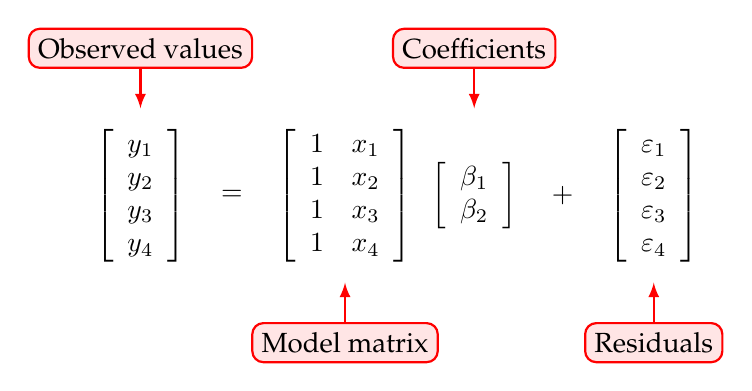
\begin{tikzpicture}
	% minimum height on nodes to align labels above components
	\begin{scope}[every node/.style={minimum height=22mm}]
	\node                    (Y)  {$\left[ \begin{array}{c} y_1 \\ y_2 \\ y_3 \\ y_4 \end{array}\right]$};
	\node [right= 2mm of Y]  (eq) {$=$};                                     
	\node [right= 2mm of eq] (X)  {$\left[ \begin{array}{cc} 1 & x_1 \\ 1 & x_2 \\ 1 & x_3 \\ 1 & x_4 \end{array}\right]$};
	\node [right= 0mm of X]  (b)  {$\left[ \begin{array}{c} \beta_1 \\ \beta_2 \end{array}\right]$};
	\node [right= 2mm of b]  (pl) {$+$};
	\node [right= 2mm of pl] (e)  {$\left[ \begin{array}{c} \varepsilon_1 \\ \varepsilon_2 \\ \varepsilon_3 \\ \varepsilon_4 \end{array}\right]$};
	\end{scope}
	
	\begin{scope}[every node/.style={rounded corners, draw, fill=red!10},
	              every path/.style={latex-, draw=red, thick, fill=red}]
	
	
		\node [above= 5mm of Y] (obs) {Observed values};
		\node [below= 5mm of X] (mat) {Model matrix};
		\node [above= 5mm of b] (coe) {Coefficients};
		\node [below= 5mm of e] (res) {Residuals};
		\draw (Y) -- (obs);
		\draw (X) -- (mat);
		\draw (b) -- (coe);
		\draw (e) -- (res);
	
	
	\end{scope}
	
	\end{tikzpicture}
	\end{center}
\end{frame}

%%%%%%%%%%%%%%%%%%%%%%%%%%%%%%%%%%%%%%%%%%%%%%%%%%%%%%%%%%%%%

\begin{frame}{The maths magic under the hood}

\begin{center}

{\LARGE $\mathbf{Y} = \mathbf{X \beta  +  \varepsilon}$}

\vspace{5mm}

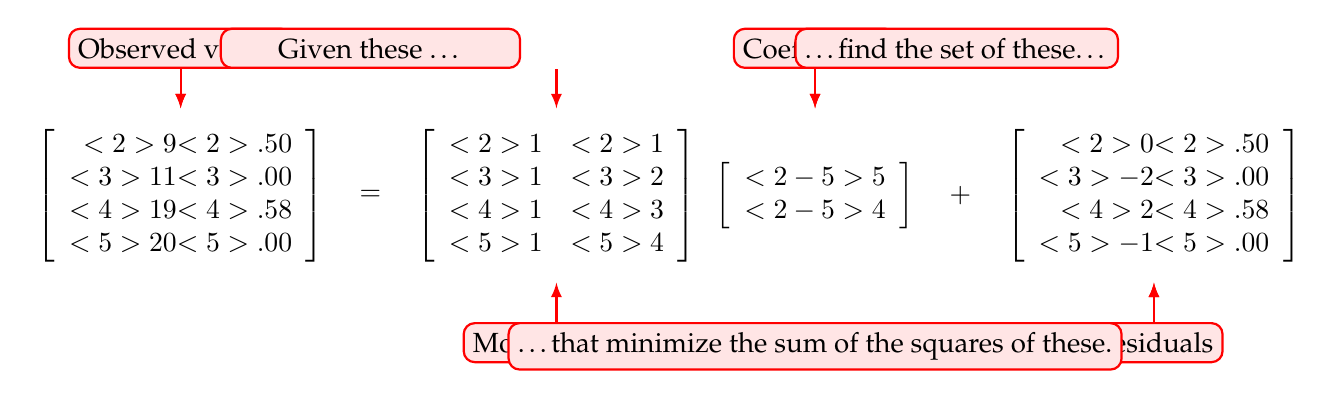
\begin{tikzpicture}
% minimum height on nodes to align labels above components
\begin{scope}[every node/.style={minimum height=22mm}]
\node                    (Y)  {$\left[ \begin{array}{r@{}l}
 								   \alert<2>  {9} & \alert<2>{.50} \\ 
								   \alert<3> {11} & \alert<3> {.00} \\ 
                                    \alert<4> {19} & \alert<4> {.58} \\ 
                                    \alert<5> {20} & \alert<5> {.00}  \end{array}\right]$};
\node [right= 2mm of Y]  (eq) {$=$};                                     
\node [right= 2mm of eq] (X)  {$\left[ \begin{array}{cc} \alert<2>{1} & \alert<2>{1} \\
                                     \alert<3>{1} & \alert<3>{2} \\ 
                                     \alert<4>{1} & \alert<4>{3} \\ 
                                     \alert<5>{1} & \alert<5>{4} \\ \end{array}\right]$};
\node [right= 0mm of X]  (b)  {$\left[ \begin{array}{c} \alert<2-5>{5} \\ 
                                    \alert<2-5>{4} \end{array}\right]$};
\node [right= 2mm of b]  (pl) {$+$};
\node [right= 2mm of pl] (e)  {$\left[ \begin{array}{r@{}l} 
								   \alert<2>  {0} & \alert<2>{.50} \\ 
								   \alert<3> {-2} & \alert<3> {.00} \\ 
                                    \alert<4>  {2} &\alert<4> {.58} \\ 
                                    \alert<5> {-1} & \alert<5> {.00}  \end{array}\right]$};
\end{scope}

\begin{scope}[every node/.style={rounded corners, draw, fill=red!10},
              every path/.style={latex-, draw=red, thick, fill=red}]

\onslide<1-5>{
	\node [above= 5mm of Y] (obs) {Observed values};
	\node [below= 5mm of X] (mat) {Model matrix};
	\node [above= 5mm of b] (coe) {Coefficients};
	\node [below= 5mm of e] (res) {Residuals};
	\draw (Y) -- (obs);
	\draw (X) -- (mat);
	\draw (b) -- (coe);
	\draw (e) -- (res);
}

\onslide<6>{
	\node [above= 5mm of eq, minimum width=38mm] (given) {Given these \ldots};
	\node [above= 5mm of b, xshift=18mm] (find) {\ldots find the set of these\ldots};
	\node [below= 5mm of b] (min)  {\ldots that minimize the sum of the squares of these.};

	\draw (Y.north) -- (Y.north |- given.south);
	\draw (X.north) -- (X.north |- given.south);
	\draw (b.north) -- (b.north |- find.south);
	\draw (e.south) -- (e.south |- min.north);   
}

\end{scope}

\end{tikzpicture}
\end{center}
\end{frame}

%%%%%%%%%%%%%%%%%%%%%%%%%%%%%%%%%%%%%%%%%%%%%%%%%%%%%%%%%%%%%

\begin{frame}{The maths magic under the hood}

\begin{center}

{\LARGE $\mathbf{\hat{Y}} = \mathbf{X \beta }$}

\vspace{5mm}

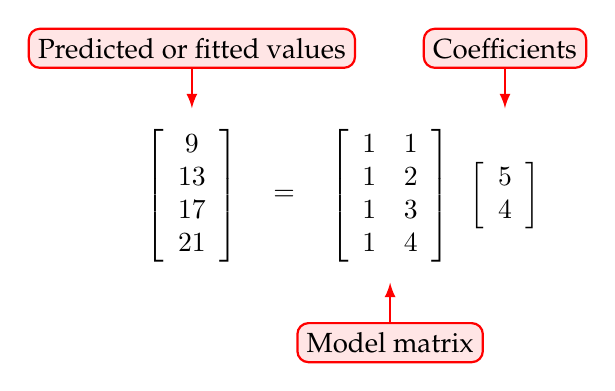
\begin{tikzpicture}
% minimum height on nodes to align labels above components
\begin{scope}[every node/.style={minimum height=22mm}]
\node                    (Y)  {$\left[ \begin{array}{c} {9} \\ 
                                     {13} \\ 
                                     {17} \\ 
                                     {21} \\ \end{array}\right]$};
\node [right= 2mm of Y]  (eq) {$=$};                                     
\node [right= 2mm of eq] (X)  {$\left[ \begin{array}{cc} {1} & {1} \\
                                     {1} & {2} \\ 
                                     {1} & {3} \\ 
                                     {1} & {4} \\ \end{array}\right]$};
\node [right= 0mm of X]  (b)  {$\left[ \begin{array}{c} {5} \\ 
                                    {4} \end{array}\right]$};
\end{scope}

\begin{scope}[every node/.style={rounded corners, draw, fill=red!10},
              every path/.style={latex-, draw=red, thick, fill=red}]

	\node [above= 5mm of Y] (obs) {Predicted or fitted values};
	\node [below= 5mm of X] (mat) {Model matrix};
	\node [above= 5mm of b] (coe) {Coefficients};
	\draw (Y) -- (obs);
	\draw (X) -- (mat);
	\draw (b) -- (coe);
	
\end{scope}

\end{tikzpicture}
\end{center}
\end{frame}

%%%%%%%%%%%%%%%%%%%%%%%%%%%%%%%%%%%%%%%%%%%%%%%%%%%%%%%%%%%%%
\begin{frame}{Predicted values and Residuals}

\begin{columns}[T]

	\column{0.5\textwidth}
		\includegraphics[width=\textwidth]{Predicted.pdf}
		
	\column{0.5\textwidth}
		\begin{align*}
		  \hat{y}  &= \beta_1 + \beta_2 x  \\
		  \\
		  9  &= 5 + 4 \times 1 \\
		  13 &= 5 + 4 \times 2 \\
		  17 &= 5 + 4 \times 3 \\
		  21 &= 5 + 4 \times 4  
		\end{align*}
\end{columns}		
\end{frame}

%%%%%%%%%%%%%%%%%%%%%%%%%%%%%%%%%%%%%%%%%%%%%%%%%%%%%%%%%%%%%


\section{Is a linear model appropriate?}

%%%%%%%%%%%%%%%%%%%%%%%%%%%%%%%%%%%%%%%%%%%%%%%%%%%%%%%%%%%%%

\begin{frame}{Fitting a linear model: Assumptions}

\begin{itemize}\itemsep20pt
\item Linear models are fitted with the following assumptions:
\begin{itemize}
\item No measurement error in explanatory variables
\item The explanatory variables are not very highly (inter-) correlated
\item \color<2>{red} The model has constant normal variance
\end{itemize}
\item {\bf If these assumptions are not met, the model can be very wrong}
\item The first two you will should consider {\it before} even fitting a linear model
\item<2> The last one needs can be tested {\it after} fitting a linear model
\end{itemize}

\end{frame}

%%%%%%%%%%%%%%%%%%%%%%%%%%%%%%%%%%%%%%%%%%%%%%%%%%%%%%%%%%%%%

\begin{frame}{`The model has constant normal variance'}
\begin{columns}[T]

	\column{0.5\textwidth}
		\includegraphics[height=72mm]{ResidDemo.pdf}
		
	\column{0.5\textwidth}
		\begin{itemize}
		\item The data have a similar spread around any predicted point in the model
		\vspace{2cm}
		\item Overall, the residuals are {\it normally distributed}: mostly small but a few larger values
        \item Points {\it should} be spaced so as to to best capture the normal (gaussian) curve
		\end{itemize}
		
\end{columns}
\end{frame}

%%%%%%%%%%%%%%%%%%%%%%%%%%%%%%%%%%%%%%%%%%%%%%%%%%%%%%%%%%%%%

\begin{frame}{Checking if the linear model is appropriate}

\includegraphics[width=\textwidth]{ConstantVarianceMods.pdf}

\begin{itemize}[<+->]
\item All these three linear model fits appropriate for the data? Are assumptions of the linear model fit satisfied?
\pause
\begin{itemize}[<+->]\itemsep6pt
    \item The spread of the real data around the fitted line (fitted values) is about the same across the x-axis -- good
    \item But are the residuals normally distributed?
\end{itemize}
\end{itemize}

\end{frame}

%%%%%%%%%%%%%%%%%%%%%%%%%%%%%%%%%%%%%%%%%%%%%%%%%%%%%%%%%%%%%

\begin{frame}{Diagnostics for a fitted linear model}
        
\begin{itemize}[<+->]\itemsep6pt
    \item \it The spread of the real data around the fitted line (fitted values) is about the same across the x-axis\\ \pause
    
    \includegraphics[width=0.95\textwidth]{FitResid.pdf}

    \pause 
    \item That is, the residuals have about the same spread irrespective of the fitted values 
    \item The three numbered points in each plot are the three most `badly behaved' data points.
    \begin{itemize}
        \item Each number is the datum's row number in the R data frame 
    \end{itemize}
\end{itemize}

\end{frame}

%%%%%%%%%%%%%%%%%%%%%%%%%%%%%%%%%%%%%%%%%%%%%%%%%%%%%%%%%%%%%

\begin{frame}{Diagnostics for a fitted linear model}

\begin{itemize}[<+->]\itemsep6pt
    \item \it Are the residuals normally distributed?\\ \pause

    \includegraphics[width=0.95\textwidth]{QQNorm.pdf}

    \pause 
    \item Residuals from the first (simple regression) and third (polynomial) model's fits show some deviations from normality at the ends (high and low ends of their distributions), but it's acceptable
    \end{itemize}

\end{frame}
    
%%%%%%%%%%%%%%%%%%%%%%%%%%%%%%%%%%%%%%%%%%%%%%%%%%%%%%%%%%%%%

\begin{frame}{Three bad linear model fits}

\includegraphics[width=\textwidth]{NonConstantVarianceMods.pdf}

\begin{itemize}\itemsep6pt
\item These are three bad linear model fits
\pause 
\begin{itemize}[<+->]\itemsep6pt
    \item The data spread is not the same for all fitted values
    \item The first model clearly  spread is not the same for all fitted values
    \item Are the residuals normally distributed?
\end{itemize}
\end{itemize}

\end{frame}

%%%%%%%%%%%%%%%%%%%%%%%%%%%%%%%%%%%%%%%%%%%%%%%%%%%%%%%%%%%%%

\begin{frame}{Diagnostics for a (badly) fitted linear model}

\includegraphics[width=0.95\textwidth]{BadFitResid.pdf}

\pause

\includegraphics[width=0.95\textwidth]{BadQQNorm.pdf}

%% TODO - add labels

\end{frame}

%%%%%%%%%%%%%%%%%%%%%%%%%%%%%%%%%%%%%%%%%%%%%%%%%%%%%%%%%%%%%

\begin{frame}{Is a linear model appropriate?}

\begin{center} 
    \Huge
Plot the data!\\
Plot the residuals!
\end{center}

\end{frame}

%%%%%%%%%%%%%%%%%%%%%%%%%%%%%%%%%%%%%%%%%%%%%%%%%%%%%%%%%%%%%

\section{Is a linear model explanatory?}

%%%%%%%%%%%%%%%%%%%%%%%%%%%%%%%%%%%%%%%%%%%%%%%%%%%%%%%%%%%%%% 
\begin{frame}{How explanatory is the fitted linear model?}

\begin{center}
\begin{itemize}[<+->]\itemsep20pt
\item The role of $F$ and $t$ tests in Linear Model fitting
\item Significance of {\it Terms}: $F$ test
\begin{itemize}
    \item Does the model explain enough variation?
    \item Does each term explain enough variation?
\end{itemize}
\item Significance of {\it Coefficients}: $t$ tests
\begin{itemize}
    \item Are the coefficients different from zero?
\end{itemize}
\end{itemize}

\end{center}
\end{frame}

% %%%%%%%%%%%%%%%%%%%%%%%%%%%%%%%%%%%%%%%%%%%%%%%%%%%%%%%%%%%%%%%%%%%%%

\begin{frame}{Is the fitted linear model significant?: $F$ test}

\begin{itemize}[<+->]\itemsep6pt

\item {\bf Total sum of squares} (TSS): Sum of the squared difference between the observed dependent variable ($y$) and the mean of $y$ ($\bar{y}$), or,		
 TSS = $\sum_{i=1}^{n}(y_i - \bar{y})^2$\\
{\it TSS tells us how much variation there is in the dependent variable}

\item {\bf Explained sum of squares} (ESS): Sum of the squared 
differences between the predicted $y$ ($\hat{y}$) and $\bar{y}$, or,
ESS = $\sum_{i=1}^{n} (\hat{y}_i - \bar{y})^2$\\

{\it ESS tells us how much of the variation in the dependent variable 
our model was able to explain}

\item {\bf Residual sum of squares} (RSS): Sum of the squared 
differences between the observed $y$ and the predicted $\hat{y}$ (residuals), or, \\

RSS = $\sum_{i=1}^{n} (\hat{y}_i - y_i)^2$\\

{\it RSS tells us how much of the variation in the dependent variable 
our model could not explain}

\item Of course, TSS = ESS + RSS

\end{itemize}

\end{frame}

%%%%%%%%%%%%%%%%%%%%%%%%%%%%%%%%%%%%%%%%%%%%%%%%%%%%%%%%%%%%%%%%%%%%%
\begin{frame}{Null vs. over-specified models: two endpoints}

    \begin{columns}[T]
	\column{0.5\textwidth}
		\includegraphics[height=72mm]{NullSaturated.pdf}

	\column{0.5\textwidth}
		\begin{itemize}
		\item The null model ($H_0$)
		\item Nothing is going on
		\item Biggest possible residuals
		\item Residual sum of squares (RSS) is as big as it can be
		\vspace{1cm}
		\item The saturated model
		\item One coefficient per data point
		\item RSS is zero - all the sums of squares are now explained (ESS)
		\end{itemize}
		
\end{columns}
\end{frame}
%%%%%%%%%%%%%%%%%%%%%%%%%%%%%%%%%%%%%%%%%%%%%%%%%%%%%%%%%%%%%%%%%%%%%

\begin{frame}{The `right' (interesting) model}

    \centerline{\includegraphics[height=0.5\textheight]{Intermediate.pdf}}

    \begin{itemize}\itemsep6pt
    \item Added a term with three levels
    \item Some but not all of the residual sums of squares are explained
    \item Is this enough to be interesting?
    \end{itemize}		

\end{frame}

%%%%%%%%%%%%%%%%%%%%%%%%%%%%%%%%%%%%%%%%%%%%%%%%%%%%%%%%%%%%%%%%%%%%%
\begin{frame}{$F$ statistic of the fitted Linear Model}

\begin{center}

	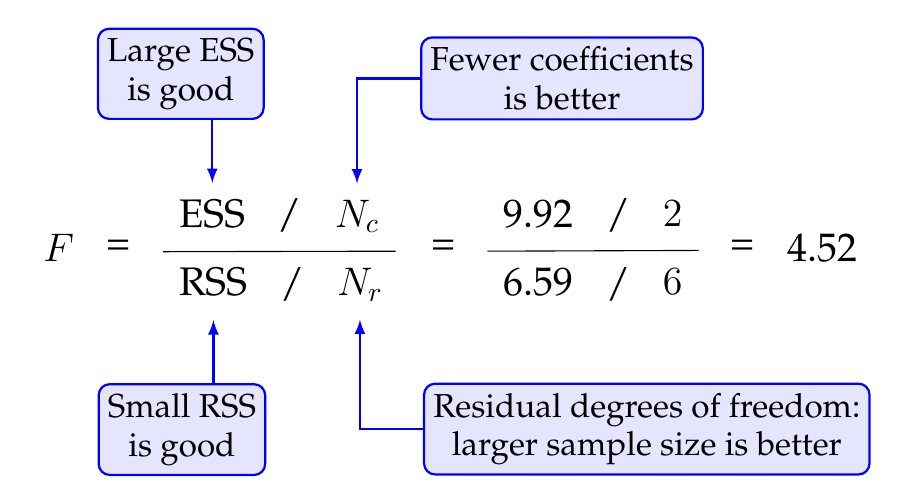
\begin{tikzpicture}[every node/.style={ text depth=1mm, inner sep=2mm,font=\Large}, node distance=0mm]
	
	\node (stat) {$F$};
	\node (eq1) [right= of stat] {=};

	\matrix (ratio1) [right=of eq1,ampersand replacement=\&] {
		\node (ESS) {ESS}; \node(div1) [right=of ESS] {/}; \node (Nc) [right= of div1]{$N_c$} ; \\ 
		\node (RSS) 	{RSS}; \node(div2) [right=of RSS]{/}; \node (Nr) [right= of div2]{$N_r$} ;\\
	};

	\draw (ESS.south west) -- (Nc.south east);
	\node (eq2) [right= of ratio1] {=};

	\matrix (ratio2)[right=of eq2,ampersand replacement=\&] {
		\node (ESSn) {9.92}; \node(div3) [right=of ESSn] {/}; \node (Ncn) [right= of div3]{$2$} ; \\ 
		\node (RSSn) {6.59}; \node(div4) [right=of RSSn]{/}; \node (Nrn) [right= of div4]{$6$} ;\\
	};

	\draw (ESSn.south west) -- (Ncn.south east);
	
	\node (eq3) [right= of ratio2] {=};
	\node (res) [right= of eq3] {4.52};
	
	\begin{scope} [every node/.style={fill=blue!10, draw=blue, font=\large, rounded corners, align=center},
                   every path/.style={latex-,  thick, draw=blue}]
    \pause
    \node (ESSGood)  [above=of ESS, yshift=8mm, xshift=-4mm] {Large ESS \\ is good};	
	\draw [blue] (ESS.north) -- (ESS.north |- ESSGood.south);
    \pause 
    \node (RSSGood)  [below=of RSS, yshift=-8mm, xshift=-4mm] {Small RSS \\ is good};	
	\draw  [blue](RSS.south) -- (RSS.south |- RSSGood.north);
    \pause 
    \node (NcGood)  [above=of Nc, yshift=8mm, xshift=8mm, anchor=south west] {Fewer coefficients \\ is better};	
    \draw [blue] (Nc.north) |- (NcGood.west);
    \pause 
    \node (NrGood)  [below=of Nr, yshift=-8mm, xshift=8mm, anchor=north west] {Residual degrees of freedom:\\ larger sample size is better};	
	\draw [blue] (Nr.south) |- (NrGood.west);
	
	\end{scope}
	
	\end{tikzpicture}

\end{center}

\end{frame}

%%%%%%%%%%%%%%%%%%%%%%%%%%%%%%%%%%%%%%%%%%%%%%%%%%%%%%%%%%%%%%%%%%%%%
\begin{frame}{What it really means: $F$ value by chance?}

\begin{center}
    \it What would be the distribution of $F$ if nothing is going on?\\
    \pause
    \includegraphics[width=\textwidth]{F_extremes.pdf}
\end{center}

\pause 
\begin{itemize}[<+->]\itemsep6pt
    \item Simulate 10,000 datasets where nothing is going on ($H_0$ is true)
    \item Calculate $F$ for each random dataset under $H_1$
    \item $H_1$ typically has a low $F$ -- but sometimes it is high {\it by chance} 
\end{itemize}

\end{frame}

%%%%%%%%%%%%%%%%%%%%%%%%%%%%%%%%%%%%%%%%%%%%%%%%%%%%%%%%%%%%%%%%%%%%%

\begin{frame}{What it really means: $F$ value by chance?}

% %% TODO: use timeline to only embed the axes once

\centerline{\animategraphics[height=0.5\textheight, 
                 %autoplay, %controls, %palindrome, 
                %  timeline=FAnimate.txt, 
                 buttonsize=1em]{12}{FAnimate}{}{}}

\begin{itemize}[<+->]\itemsep6pt
\item In our possibly interesting model, $F = 4.52$
\item 95\% of the random data sets have $F\le 5.5$
\item A model this good would be found by chance 1 in 16 times (p$=0.063$)
\item Close, but not quite interesting (significant) enough!
\end{itemize}

\end{frame}

%%%%%%%%%%%%%%%%%%%%%%%%%%%%%%%%%%%%%%%%%%%%%%%%%%%%%%%%%%%%%%%%%%%%%
\begin{frame}{Are the coefficients different from zero?}

\begin{center}

	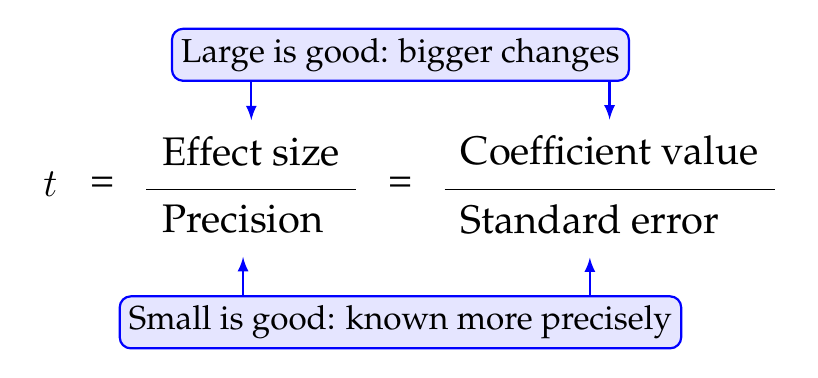
\begin{tikzpicture}[every node/.style={ text depth=1mm, inner sep=2mm,font=\Large}, node distance=0mm]
	
	\node (stat) {$t$};
	\node (eq1) [right= of stat] {=};

	\matrix (ratio1) [right=of eq1,ampersand replacement=\&] {
		\node (diff) {Effect size}; \\ 
		\node (prec) 	{Precision}; \\
	};
	\draw (diff.south west) -- (diff.south east);
	
	\node (eq2) [right= of ratio1] {=};

	\matrix (ratio2) [right=of eq2,ampersand replacement=\&] {
		\node (val) {Coefficient value}; \\ 
		\node (se) 	{Standard error}; \\
	};
	\draw (val.south west) -- (val.south east);
	
	\begin{scope} [every node/.style={fill=blue!10, draw=blue, font=\large, rounded corners, align=center},
                   every path/.style={latex-,  thick, draw=blue}]

    \pause 
    \node (esgood)  [above=of eq2, yshift=10mm ] {Large is good: bigger changes};	
	\draw [blue] (diff.north) -- (diff.north |- esgood.south);
	\draw [blue] (val.north) -- (val.north |- esgood.south);
    
    \pause 
    \node (precgood)  [below=of eq2, yshift=-10mm] {Small is good: known more precisely};	
	\draw [blue] (prec.south) -- (prec.south |- precgood.north);
	\draw [blue] (se.south) -- (se.south |- precgood.north);	
		
	\end{scope}
	
	\end{tikzpicture}
\end{center}

\pause 
\begin{itemize}[<+->] \itemsep6pt
    \item The value of a coefficient in a model is an {\it effect size}
    \item How much does changing that predictor variable change the response variable?
    \item The {\it standard error} estimates how precisely we know the value
\end{itemize}

\end{frame}
%%%%%%%%%%%%%%%%%%%%%%%%%%%%%%%%%%%%%%%%%%%%%%%%%%%%%%%%%%%%%%%%%%%%%

\begin{frame}{Variation in effect size and precision}
	
\centerline{\includegraphics[height=75mm]{T_examples.pdf}}

\end{frame}

%%%%%%%%%%%%%%%%%%%%%%%%%%%%%%%%%%%%%%%%%%%%%%%%%%%%%%%%%%%%%%%%%%%%%
\begin{frame}{What it really means: $t$ values by chance}

\begin{center}
    \it What is the distribution of $t$ if nothing is going on?\\
    \pause
    \includegraphics[width=\textwidth]{t_extremes.pdf}
\end{center}

\pause
\begin{itemize}[<+->]\itemsep6pt
\item Simulate 10,000 datasets where nothing is going on ($H_0$ is true)
\item Calculate $t$ for each random dataset under $H_1$
\item $H_1$ typically has a $t$ near zero but can be strongly positive or negative {\it by chance}
\end{itemize}

\end{frame}

%%%%%%%%%%%%%%%%%%%%%%%%%%%%%%%%%%%%%%%%%%%%%%%%%%%%%%%%%%%%%%%%%%%%%

\begin{frame}{Distribution of $t$}

% %% animate directly from a multipage pdf - this is rather sweet!
% %% this is also over-engineered using timeline to only embed the axes once!

\centerline{\animategraphics[height=0.5\textheight, 
                 %autoplay, %controls, %palindrome, 
                %  timeline=tAnimate.txt, 
                 buttonsize=1em]{12}{tAnimate}{}{}}

\pause 
\begin{itemize}[<+->] \itemsep6pt
    \item 95\% of the random data sets have $t\le \pm 2.09$
    \item Only the two higher precision models are expected to occur less than 1 time in 20 by chance.
\end{itemize}

\end{frame}

%%%%%%%%%%%%%%%%%%%%%%%%%%%%%%%%%%%%%%%%%%%%%%%%%%%%%%%%%%%%%%%%%%%%%

\begin{frame}{Some more examples of linear model fitting}

\includegraphics[width=\textwidth]{ANOVA_null.pdf}

\begin{itemize}[<+->]\itemsep6pt
\item The null hypothesis ($H_0$): Nothing is going on (model is just $\beta_1$!)
\item The residuals (and therefore, RSS) will get {\it smaller} as we include more terms to the model
\item {\it How much smaller is enough?}
\end{itemize}

\end{frame}

%%%%%%%%%%%%%%%%%%%%%%%%%%%%%%%%%%%%%%%%%%%%%%%%%%%%%%%%%%%%%%%%%%%%%

\begin{frame}{Some more examples of linear model fitting}

    \begin{center}
        {\it First try: Add one continuous term}\\

        \includegraphics[width=\textwidth]{ANOVA_mod.pdf}
    \end{center}

\begin{itemize}[<+->]\itemsep10pt
\item Fitted an {\it alternative} model ($H_1$) using a predictor variable $x$
\item i.e., Added one term ($x$) to the model to give ($H_1$)
\item Do we reject $H_0$ and accept this new model?
\end{itemize}

\end{frame}

%%%%%%%%%%%%%%%%%%%%%%%%%%%%%%%%%%%%%%%%%%%%%%%%%%%%%%%%%%%%%%%%%%%%%

\begin{frame}{Some more examples of linear model fitting}

    \begin{center}
        {\it Second try: Add one continuous term}\\

        \includegraphics[width=\textwidth]{ANOVA_mod2.pdf}
    \end{center}

\begin{itemize}[<+->]\itemsep6pt
    \item Fitted another model ($H_2$) with continuous predictor $x$ and factor $f$
    \item The RSS gets still smaller 
    \item Is this {\it even} better than $H_1$?
\end{itemize}

% \footnotetext[1]{Note that we've added one term ($f$) but two coefficients ($f_b$ and $f_c$) --- recall where the baseline level is}

\end{frame}

%%%%%%%%%%%%%%%%%%%%%%%%%%%%%%%%%%%%%%%%%%%%%%%%%%%%%%%%%%%%%%%%%%%%%

\begin{frame}{Compare the three models}

\begin{table}[htdp]
	\begin{center}
		\begin{tabular}{ccccc}
				&  & Model A & Model B & Model C \\
		\hline
		$H_0 $ & Unexplained SS & 241.97 & 185.02 & 259.80 \\
		       & Explained SS   & 0      & 0      &    0   \\
		$H_1 $ & Unexplained SS & 241.97 & 173.21 & 62.95 \\
		       & Explained SS   & 0.00  & 11.81 & 196.85 \\
		$H_2 $ & Unexplained SS & 238.07 & 123.75 & 25.05 \\
		       & Explained SS   & 3.9  & 61.27 & 234.75 \\
        \hline
    \end{tabular}
\end{center}
\end{table}

\begin{itemize}[<+->]\itemsep6pt
    \item Which model would you choose between $H_1$ and $H_2$?
    \item Every alternative model is an {\it alternative hypothesis}
\end{itemize}
    
\end{frame}

%%%%%%%%%%%%%%%%%%%%%%%%%%%%%%%%%%%%%%%%%%%%%%%%%%%%%%%%%%%%%%%%%%%%%

\begin{frame}{Linear Models: Summary}

    \begin{itemize}\itemsep12pt
        \item Linear models predict a continuous response variable
        \item A LM is a sum of terms that are linear in the coefficients capturing the effect sizes of explanatory variables
        \item LMs are fitted using (ordinary) least squares --- minimizes sum of squared residuals
        \item Need to check if the fitted LM is appropriate
        \item Then check if the LM is explanatory
        \item Fitting alternative LMs = Testing alternative hypotheses
    \end{itemize}
    
    \end{frame}
    
%%%%%%%%%%%%%%%%%%%%%%%%%%%%%%%%%%%%%%%%%%%%%%%%%%%%%%%%%%%%%%%%%%%%
	
% \begin{frame}{Categorical variables}
% \begin{columns}[T]

% \column{0.5\textwidth}
% 	\includegraphics[width=\textwidth]{Anova.pdf}
	
% \column{0.5\textwidth}
% 	Features of categorical variables\\
% 	\begin{itemize}
% 		\item Also called {\it factors}
% 		\item Have a set of discrete {\it levels}
% 		\item We want to model {\it differences} between levels
% 		\item The least squares estimate for a level is simply the {\it mean} within the level
% 		\item How do we include this in the linear model?
% 	\end{itemize}
% \end{columns}		
% \end{frame}

%%%%%%%%%%%%%%%%%%%%%%%%%%%%%%%%%%%%%%%%%%%%%%%%%%%%%%%%%%%%%%%%%%%%
% \frame
% {\frametitle{Contrasts}
% 
% \begin{itemize}
% \item Many possible differences between levels ({\it contrasts})
% \item For 4 levels, the possible contrasts between:
% \begin{itemize}
% \item two levels
% \item a pair of levels and a third level
% \item two pairs of levels
% \item one level and the remaining three levels
% \end{itemize}
% \item Each {\it contrast} represents a possible hypothesis.
% \end{itemize}
% \vspace{3mm}
% 
	% \begin{tikzpicture}
	% 
	% \newcommand{\bb}{\node [circle,  fill=blue, inner sep=0.5mm]{} ;}
	% \newcommand{\rr}{\node [circle,  fill=red, inner sep=0.5mm]{} ;}
	% 
	% \matrix (contrasts) [matrix of nodes, ampersand replacement=\&,  BEAMER hijacks straight &
	                     % row sep=1mm, column sep=2.5mm, 
	                     % nodes={circle, fill=black!35, inner sep=0.5mm}, nodes in empty cells]
	% {
		    % \&     \& \bb \&     \& \rr \& \rr \& [4mm]  {a}{b}
		    % \& \rr \&     \& \rr \& \bb \& \bb \&     \& \rr \& \bb \& \bb \& [4mm]  {ab}{c}
	    % \rr \& \rr \&  \bb \& [4mm]  {ab}{cd}
	    % \rr \& \bb \& \bb \& \bb \\[1.5mm]  {abc}{d}
		    % \& \bb \&     \& \rr \&     \& \bb \& 
		% \rr \&     \& \bb \& \bb \&     \& \rr \& \bb \& \bb \& \bb \& \bb \& 
		% \rr \& \bb \& \rr \& 
		% \bb \& \rr \& \bb \& \bb \\[12mm]
		% \bb \&     \&     \& \bb \& \bb \&     \& 
		% \bb \& \bb \& \rr \&     \& \rr \&     \& \bb \& \bb \&     \& \rr \& 
		% \bb \& \rr \& \rr \& 
		% \bb \& \bb \& \rr \& \bb \\[1.5mm]
		% \rr \& \rr \& \rr \&     \&     \&     \&
	    % \bb \& \bb \& \bb \& \bb \& \bb \& \bb \& \rr \&     \& \rr \&     \& 
	    % \bb \& \bb \&  \bb \&
	    % \bb \& \bb \& \bb \& \rr \\
	% };
	% 
	%% Draw in background bars to clarify contrast sets
	% \begin{scope}[on background layer, every node/.style=
	                  % {rounded corners, inner sep=0.7mm,
	                    % fill=black!20}]
	                   % 
		 % \def\x{contrasts-1-\i}
		 % \def\y{contrasts-4-\i}
		 % \def\r{col-\i}		  
	     % \foreach \i in {1, 2, ..., 23} \node (\r) [fit=(\x) (\y)]{};
	% \end{scope}
	% 
	% \node[left=4mm of contrasts-1-1]{Treat 2};
	% \node[left=4mm of contrasts-2-1]{Treat 1};
	% \node[left=4mm of contrasts-3-1]{Manip};
     	% \node[left=4mm of contrasts-4-1]{Control};
	% 
			% \draw ([yshift=5mm] col-1.north west)   -- node[above, font=\footnotesize] {\{a\} v. \{b\}}   ([yshift=5mm] col-6.north east);
			% \draw ([yshift=-5mm] col-7.south west)  -- node[below, font=\footnotesize] {\{a,b\} v. \{c\}}   ([yshift=-5mm] col-16.south east);
			% \draw ([yshift=5mm] col-17.north west)  -- node[above, font=\footnotesize] {\{a,b\} v. \{c,d\}}   ([yshift=5mm] col-19.north east);
			% \draw ([yshift=-5mm] col-20.south west) -- node[below, font=\footnotesize] {\{a,b,c\} v. \{d\}}   ([yshift=-5mm] col-23.south east);
	% 
	% \end{tikzpicture}
% }	

%%%%%%%%%%%%%%%%%%%%%%%%%%%%%%%%%%%%%%%%%%%%%%%%%%%%%%%%%%%%%%%%%%%%%
% \begin{frame}{How to find $\beta$ \dots}
	
% 	\begin{center}
% 	\begin{tikzpicture}
	
% 	\node                     (eq1)  {=};
% 	\node [left=  2mm of eq1] (lhs1) {$\mathbf{Y}$};
% 	\node [right= 2mm of eq1] (rhs1) {$\mathbf{X \beta  +  \varepsilon}$};
% 	\node [below= 7mm of eq1] (eq2)  {=};
% 	\node [left=  2mm of eq2] (lhs2) {$\mathbf{X^T Y}$};
% 	\node [right= 2mm of eq2] (rhs2) {$\mathbf{X^T X \beta}$};
% 	\node [below= 7mm of eq2] (eq3)  {=};
% 	\node [left=  2mm of eq3] (lhs3) {$\mathbf{(X^T X )^{-1} X^T Y}$};
% 	\node [right= 2mm of eq3] (rhs3) {$\mathbf{\beta}$};
		
% 	\end{tikzpicture}
% 	\end{center}
	
% \end{frame}


%\frame
%{\frametitle{Model as a matrix - terminology}
%
%\begin{center}
%
%{\LARGE $\mathbf{Y} = \mathbf{X \beta  +  \varepsilon}$}
%
%\vspace{5mm}
%
%\begin{tikzpicture}
%% minimum height on nodes to align labels above components
%\begin{scope}[every node/.style={minimum height=22mm}]
%\node                    (Y)  {$\left[ \begin{array}{c} 
%									1.58 \\ 6.79 \\
%									4.16 \\ 6.73 \\
%									4.26 \\ 6.33 \\
%									3.18 \\ 8.73
%                                 \end{array}\right]$};
%\node [right= 2mm of Y]  (eq) {$=$};                                     
%\node [right= 2mm of eq] (X)  {$\left[ \begin{array}{cccc} 
%									1 & 0 & 0 & 0 \\  1 & 0 & 0 & 0 \\  
%									1 & 1 & 0 & 0 \\  1 & 1 & 0 & 0 \\  
%									1 & 0 & 1 & 0 \\  1 & 0 & 1 & 0 \\  
%									1 & 0 & 0 & 1 \\  1 & 0 & 0 & 1 \\ 
%                                \end{array}\right]$};
%\node [right= 0mm of X]  (b)  {$\left[ \begin{array}{c} 
%                                         \beta_1 \\ \beta_2 \\
%                                         \beta_3 \\ \beta_4 \\
%                                 \end{array}\right]$};
%                                 
%\node [right= 2mm of b]  (pl) {$+$};
%\node [right= 2mm of pl] (e)  {$\left[ \begin{array}{c} 
%                                         \varepsilon_1 \\ \varepsilon_2 \\
%                                         \varepsilon_3 \\ \varepsilon_4 \\
%                                         \varepsilon_5 \\ \varepsilon_6 \\
%                                         \varepsilon_7 \\ \varepsilon_8 \\
%                                 \end{array}\right]$};
%\end{scope}
%
%\end{tikzpicture}
%\end{center}
%}
%
%
%\frame
%{\frametitle{Categorical variables}
%\begin{columns}[T]
%
%\column{0.5\textwidth}
%	\includegraphics[width=\textwidth]{AnovaCoef.pdf}
%	
%\column{0.5\textwidth}
%\end{columns}		
%}
%
%
%
%
%\frame
%{\frametitle{Model as a matrix - terminology}
%
%\begin{center}
%
%{\LARGE $\mathbf{Y} = \mathbf{X \beta  +  \varepsilon}$}
%
%\vspace{5mm}
%
%\begin{tikzpicture}
%% minimum height on nodes to align labels above components
%\begin{scope}[every node/.style={minimum height=22mm}]
%\node                    (Y)  {$\left[ \begin{array}{c} 
%									1.58 \\ 6.79 \\
%									4.16 \\ 6.73 \\
%									4.26 \\ 6.33 \\
%									3.18 \\ 8.73
%                                 \end{array}\right]$};
%\node [right= 2mm of Y]  (eq) {$=$};                                     
%\node [right= 2mm of eq] (X)  {$\left[ \begin{array}{cccc} 
%									1 &  0.5 & -0.5 &    0 \\  1 &  0.5 & -0.5 &    0 \\  
%									1 &  0.5 &  0.5 &    0 \\  1 &  0.5 &  0.5 &    0 \\  
%									1 & -0.5 &    0 & -0.5 \\  1 & -0.5 &    0 & -0.5 \\  
%									1 & -0.5 &    0 &  0.5 \\  1 & -0.5 &    0 &  0.5 \\ 
%                                \end{array}\right]$};
%\node [right= 0mm of X]  (b)  {$\left[ \begin{array}{c} 
%                                         \beta_1 \\ \beta_2 \\
%                                         \beta_3 \\ \beta_4 \\
%                                 \end{array}\right]$};
%                                 
%\node [right= 2mm of b]  (pl) {$+$};
%\node [right= 2mm of pl] (e)  {$\left[ \begin{array}{c} 
%                                         \varepsilon_1 \\ \varepsilon_2 \\
%                                         \varepsilon_3 \\ \varepsilon_4 \\
%                                         \varepsilon_5 \\ \varepsilon_6 \\
%                                         \varepsilon_7 \\ \varepsilon_8 \\
%                                 \end{array}\right]$};
%\end{scope}
%
%\end{tikzpicture}
%\end{center}
%}
%
%
%
%\frame
%{\frametitle{Concepts}
%\begin{centering}
%  
%
%\includegraphics[width=\textwidth]{ScatterplotGroup.pdf}
%
%\end{centering}
%}
%
%\frame
%{\frametitle{Concepts}
%
%\begin{centering}
%
%\includegraphics[width=\textwidth]{CoefMarkup.pdf}
%
%\end{centering}
%
%}
%\section{Is a linear model appropriate?}
%\frame
%{\frametitle{Concepts}
%
%\begin{centering}
%
%\includegraphics[width=\textwidth]{CoefMarkup.pdf}
%
%\end{centering}
%
%}
%
%\frame
%{\frametitle{Concepts}
%
%\begin{centering}
%
%\includegraphics[width=\textwidth]{CoefMarkup.pdf}
%
%\end{centering}
%
%}

\end{document}

